\documentclass[fleqn,10pt]{article}%
\usepackage[hangul,nonfrench,finemath]{kotex}
\usepackage[HWP]{dhucs-interword}
\usehangulfontspec{ut}
\usepackage[hangul]{dhucs-setspace}
\usepackage{ifpdf}
\ifpdf
\usepackage[unicode,pdftex,colorlinks]{hyperref}
\input glyphtounicode\pdfgentounicode=1
\else
\usepackage[unicode,dvipdfm,colorlinks]{hyperref}
%\pdfmapfile{+unttf-pdftex-dhucs.map}
\fi 

\usepackage[utf8]{inputenc}
\usepackage[dvips]{color}
\usepackage{defcolor}
\usepackage{bm}
\usepackage{amsmath}
\usepackage{amsfonts}
\usepackage{amssymb}
\usepackage{tikz}
\usepackage{graphicx}%
\setlength{\topmargin}{-1.0in}
\setlength{\textheight}{9.25in}
\setlength{\oddsidemargin}{0.0in}
\setlength{\evensidemargin}{0.0in}
\setlength{\textwidth}{6.5in}
\pagestyle{plain}
\setcounter{secnumdepth}{0}
\parindent=0pt
\begin{document}

\begin{center}
\textbf{\Large 물리학 I 2022년 1학기}
\vspace{0.5cm}

\textbf{숙제 4: 뉴턴의 운동법칙 (담당교수: 김현철)}
\end{center}
\vspace{0.8cm}

\textbf{\color{red}제출기한: 2022년 3월 30일 수요일 오후 15:00시까지}
\vspace{1.0cm}



\noindent {\bf 문제 2. (20pt)} 그림~\ref{fig:2}처럼 자동차 $A$가
언덕을 내려오다가 미끄러져 빨간 신호등 앞에서 멈춰있는 자동차 $B$를
들이 받았다. 언덕의 각도가 $\theta=12.0^\circ$이고 자동차 $A$가
미끄러지기 시작할 때 두 차 사이의 간격은 $d=24.0$ m이며 그때 자동차
$A$의 속력은 $v_0=18.0\,\mathrm{m/s}$이다. 운동마찰계수가 아래와 같이
주어질 때 자동차 $A$가 자동차 $B$를 추돌하는 순간의 속력을 구하여라. 
\begin{figure}[htp]
  \centering
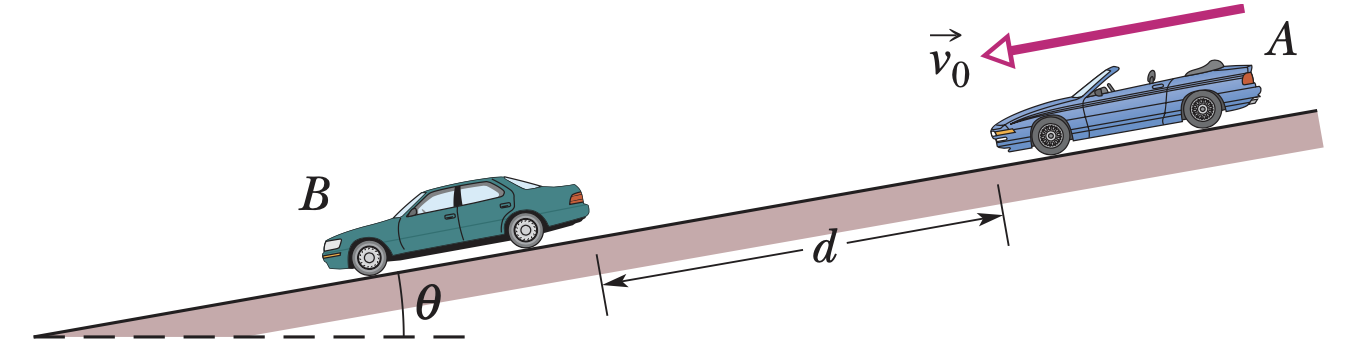
\includegraphics[scale=0.4]{hwfig4-2-20210402.png}
  \caption{문제 2}
\label{fig:2}  
\end{figure}
\begin{itemize}
\item[(가)] $\mu_k=0.600$ (마른 도로)
\item[(나)] $\mu_k=0.100$ (젖은 낙엽이 깔려있는 도로)
\end{itemize}

\noindent {\bf 풀이 : }
\begin{itemize}
  \item[(가)] 자동차 A 가 받는 힘을 자유 물체 다이어 그램으로 
표현해보자.
\begin{figure}[h]
  \centering
  \begin{tikzpicture}%\usepackage{tikz}
    \draw[rotate=12] (-2.5,0) -- (2.5,0) ;
    \draw[rotate=12] (0,-2.5) -- (0,2.5) ;
    \draw[rotate=12,blue,very thick,-latex] (0.1,0) -- (0.8,0) 
    node[black,above] {$f_k$} ;
    \draw[violet,very thick,-latex] (0,-0.1) -- (0,-2)
    node[black,left] {$F_g$} ;
    \draw[rotate=12,red,very thick,-latex] (0,0.1) -- (0,1.8)
    node[black,left] {$N$} ;
    \draw (0,-1) arc(258:270:1) 
    node[below=10,left=-4] {$\theta$}; 
  \end{tikzpicture}
  \caption{자유 물체 다이어 그램}
\end{figure}
$\mu_k=0.600$ 일 때 자동차 A 가 받는 힘을 성분 별로 분해해보면 다음과 같다.
\begin{align}
  \begin{split}
    \sum F_x&=ma=F_g\sin{\theta}-f_k,\,\,\,f_k=\mu_k N \\
    \sum F_y&=N-F_g\cos{\theta}=0.
  \end{split}
\end{align}
자동차는 받은 알짜힘 만큼 운동 에너지를 얻는다. 자동차가 받는 알짜힘은,
\begin{align}
  W = (F_g\sin{\theta}-\mu_k N)d=(F_g\sin{\theta}-\mu_kF_g\cos{\theta})d.
\end{align}
따라서 충돌 직전 속력을 $v_f$ 라 하면,
\begin{align}
  (F_g\sin{\theta}-\mu_kF_g\cos{\theta})d 
  = \frac{1}{2}mv^2_f-\frac{1}{2}mv^2_0,\,\,\,
  v_f =\sqrt{\frac{2(F_g\sin{\theta}-\mu_kF_g\cos{\theta})d}{m} 
  +v^2_0}.
\end{align}
$F_g=mg$ 이므로,
\begin{align}\label{eq:2-1}
  \begin{split}
    v_f &= \sqrt{2(\sin{\theta}-\mu_k \cos{\theta})gd 
    +v^2_0} \\
    &= \sqrt{2(\sin{12^\circ}-(0.600) \cos{12^\circ})
    (9.80\,\mathrm{m/s^2})(24.0\,\mathrm{m}) 
    +(18.0\,\mathrm{m/s})^2} \\
    &= 12.1\,\mathrm{m/s}.
  \end{split}
\end{align}
$\mu_k=0.600$ 인 경우, 자동차의 충돌 직전 속력은 $12.1\,\mathrm{m/s}$ 이다.
\item[(나)] 식 (\ref{eq:2-1}) 으로 부터 $\mu_k=0.100$ 인 경우 이므로,
\begin{align}
  \begin{split}
    v_f &= \sqrt{2(\sin{\theta}-\mu_k \cos{\theta})gd 
    +v^2_0} \\
    &= \sqrt{2(\sin{12^\circ}-(0.100) \cos{12^\circ})
    (9.80\,\mathrm{m/s^2})(24.0\,\mathrm{m}) 
    +(18.0\,\mathrm{m/s})^2} \\
    &= 19.4\,\mathrm{m/s}.
  \end{split}
\end{align}
$\mu_k=0.100$ 인 경우, 자동차의 충돌 직전 속력은 $19.4\,\mathrm{m/s}$ 이다.
\end{itemize}
\end{document}
